\documentclass[a4paper,11pt]{article}

\usepackage[T1]{fontenc}
\usepackage[utf8]{inputenc}
\usepackage[slovak]{babel}
\usepackage[margin=2.5cm]{geometry}
\usepackage{xcolor}
\usepackage{hyperref}
\usepackage{graphicx}

\title{Overovanie faktov na základe prehľadávania webu\\[0.4em]
\large Plán bakalárskeho projektu}
\author{Vladyslav Morhai\\
\small Technická univerzita v Košiciach, FEI}
\date{2026}

\begin{document}
\maketitle

\noindent\textbf{Vedúci projektu:} doc. Ing. Marián Mach, CSc.

\begin{abstract}
Práca sa zaoberá automatizovaným overovaním faktov na základe vyhľadávania
na webe. Navrhujeme modulárny pipeline, ktorý pre zadané tvrdenie vygeneruje
vyhľadávací dopyt, získa relevantné webové stránky, z ich plného textu
pomocou modelu NLI určí, či tvrdenie potvrdzujú alebo vyvracajú, a výsledky
agreguje do verdiktu s mierou istoty a zoznamom dôkazov. Agregáciu
rozširujeme o váhy dôveryhodnosti zdrojov. Systém vyhodnotíme na datasete
AVeriTeC a experimentálne overíme prínos jednotlivých častí. Ak to čas
dovolí, porovnáme ho aj s prístupom založeným na veľkom jazykovom modeli,
ktorý pracuje len s úryvkami z výsledkov vyhľadávania. Prínosom má byť
transparentnejší a na referenčných dátach vyhodnotený postup.
\end{abstract}

% ------------------------------------------------------------------
\section{Úvod a motivácia}

Rýchlosť, akou sa informácie a dezinformácie šíria v online priestore,
zvyšuje význam overovania faktov (angl. \textit{fact-checking})
\cite{guo2022survey}. Overenie jedného tvrdenia pritom môže profesionálnym
overovateľom trvať hodiny až dni \cite{guo2022survey}, preto sa výskum
zameriava na jeho automatizáciu pomocou metód spracovania prirodzeného
jazyka a strojového učenia \cite{guo2022survey}.

Overovanie tvrdení len na základe znalostí uložených v jazykovom modeli je
problematické: takýto prístup môže prenášať skreslenia z trénovania
a neumožňuje podložiť verdikt dôkazmi \cite{guo2022survey}. Veľké jazykové
modely (LLM) navyše môžu generovať presvedčivo znejúce, no nepravdivé
odpovede (halucinácie). Preto vznikajú prístupy, ktoré odpoveď modelu opierajú
o výsledky vyhľadávania na webe, napríklad agent opísaný v \cite{nath-agent}.
V tomto riešení však chýba vyhodnotenie kvality verdiktov na dátach aj
posúdenie dôveryhodnosti použitých zdrojov.

Cieľom tohto projektu je navrhnúť a implementovať systém, ktorý pre zadané
tvrdenie vyhľadá relevantné webové zdroje, určí, či ich obsah tvrdenie
potvrdzuje alebo vyvracia, a zostaví z toho verdikt s dôkazmi. Ak to čas
dovolí, porovnáme ho s prístupom, v ktorom verdikt určuje LLM nad úryvkami
z výsledkov vyhľadávania \cite{nath-agent}.

% ------------------------------------------------------------------
\section{Cieľ projektu}

Hlavným cieľom projektu je navrhnúť, implementovať a vyhodnotiť systém na
overovanie faktov, ktorý pre zadané tvrdenie vyhľadá relevantné zdroje na
webe, určí ich vzťah k tvrdeniu a zostaví z neho verdikt s dôkazmi.

Na dosiahnutie hlavného cieľa sú stanovené tieto čiastkové ciele:
\begin{enumerate}
  \item Preštudovať existujúce prístupy k automatizovanému overovaniu
        faktov, najmä riešenia založené na vyhľadávaní na webe a na
        veľkých jazykových modeloch.
  \item Navrhnúť a implementovať modulárny pipeline: generovanie
        vyhľadávacieho dopytu, vyhľadávanie na webe, sťahovanie a čistenie
        plného textu stránok, určenie vzťahu medzi tvrdením a textom
        pomocou modelu NLI a agregácia výsledkov do verdiktu.
  \item Rozšíriť agregáciu o váhy dôveryhodnosti zdrojov.
  \item Vyhodnotiť systém na datasete AVeriTeC pomocou štandardných metrík
        a overiť prínos jednotlivých častí systému.
  \item Ak to čas dovolí, porovnať výsledky systému s prístupom
        založeným na LLM podľa \cite{nath-agent} na rovnakej množine
        tvrdení.
\end{enumerate}

% ------------------------------------------------------------------
\section{Prehľad existujúcich riešení}

Podľa \cite{guo2022survey} sa automatizované overovanie faktov člení na
tri etapy: detekciu tvrdení, vyhľadanie dôkazov a overenie tvrdenia, ktoré
zahŕňa predikciu verdiktu a tvorbu zdôvodnenia. Táto kapitola zhŕňa
datasety, modely a prístupy k jednotlivým etapám, ktoré sú relevantné pre
navrhované riešenie, a nakoniec stručne rozoberá, nakoľko je riešenie
závislé od jazyka.

\subsection{Datasety}

Dataset FEVER \cite{thorne2018fever}\footnote{\url{https://fever.ai/dataset/fever.html}} obsahuje približne 185\,000 tvrdení
vytvorených úpravou viet z Wikipédie. Každé tvrdenie je označené ako
Supported, Refuted alebo NotEnoughInfo a pri prvých dvoch triedach je
zaznamenaná aj veta, ktorá slúži ako dôkaz. Tvrdenia sú však umelé
a overujú sa voči Wikipédii, nie voči otvorenému webu. Tieto nedostatky
rieši dataset AVeriTeC \cite{schlichtkrull2023averitec}\footnote{\url{https://fever.ai/dataset/averitec.html}}, ktorý obsahuje
4\,568 reálnych tvrdení z fact-checkov 50 organizácií. Ku každému tvrdeniu
patria otázky a odpovede podložené dôkazmi dostupnými online a textové
zdôvodnenie verdiktu. Autori sa pri anotácii snažili vylúčiť dôkazy
zverejnené až po vzniku tvrdenia, no zaručujú to len približne. K trom
triedam FEVER pridáva štvrtú: protichodné dôkazy alebo výber len
vhodných faktov (angl. \textit{conflicting evidence/cherry-picking}).
Dataset je nevyvážený, pretože fact-checkeri vyberajú najmä nepravdivé
alebo zavádzajúce tvrdenia, a obsahuje len anglické tvrdenia. Autori
spolu s datasetom publikovali aj základný systém (angl. \textit{baseline}),
ktorý ďalej nazývame \textit{základný systém AVeriTeC}; samotný dataset
a tento systém sú dve odlišné veci.

Pre slovenčinu existuje dataset výrokov z Demagog.sk\footnote{\url{https://huggingface.co/datasets/NaiveNeuron/DemagogSK}}
s približne 20\,000 výrokmi so štyrmi triedami verdiktov, ku ktorým sú
pripojené texty fact-checkov a odkazy na použité zdroje. Nemá však
štruktúru otázok a odpovedí s dôkazmi z webu ako AVeriTeC.

\subsection{Modely pre odvodzovanie z textu (NLI)}

Overenie tvrdenia voči textu možno formulovať ako úlohu odvodzovania
z textu (angl. \textit{natural language inference}, NLI): model určí, či
text tvrdenie potvrdzuje (\textit{entailment}), vyvracia
(\textit{contradiction}) alebo sa ho netýka (\textit{neutral})
\cite{guo2022survey}. Modely pre túto úlohu vznikajú dotrénovaním
predtrénovaného jazykového modelu na korpusoch ako MultiNLI.
Moderným základom takýchto modelov je architektúra DeBERTa
\cite{he2021deberta} a jej vylepšená verzia DeBERTaV3
\cite{he2023debertav3}, ktorej veľká verzia dosiahla na
benchmarku GLUE priemerné skóre 91,37~\%, čo je o 1,37~\% viac než pôvodná
DeBERTa. Základný systém AVeriTeC \cite{schlichtkrull2023averitec} používa
podobný princíp: dotrénovaný model BERT-large označí každý
pár otázka--odpoveď ako podporujúci, vyvracajúci alebo irelevantný a verdikt
sa určí z týchto označení. Tento prístup však zlyhával pri triede
protichodných dôkazov, pretože otázky len dopĺňajúce kontext model často
chybne označil ako vyvracajúce.

\subsection{Detekcia tvrdení a dôveryhodnosť zdrojov}

Prvou etapou je detekcia tvrdení, ktoré stoja za overenie. Systém
ClaimBuster \cite{hassan2017claimbuster} v texte vyhľadáva overiteľné
faktické tvrdenia. Táto etapa nie je súčasťou projektu, vstupom je už
vybrané tvrdenie. Dôveryhodnosť zdroja, ktorú využíva rozšírená agregácia,
sa skúma samostatne: práca \cite{baly2018factuality} predikuje
faktickú spoľahlivosť a politické skreslenie spravodajských zdrojov ako
celku, nie jednotlivých článkov. Podobne chceme dôveryhodnosť priraďovať
zdroju (doméne), nie jednotlivému textu.

\subsection{Prístupy založené na LLM a vyhľadávaní}

Veľké jazykové modely (LLM) dokážu tvrdenie posúdiť aj bez dodatočných
dokumentov, no môžu si vymýšľať fakty a verdikt nemožno podložiť zdrojom.
Preto sa využíva generovanie rozšírené o vyhľadávanie (angl.
\textit{retrieval-augmented generation}, RAG): model najprv dostane
dokumenty nájdené k otázke a odpovedá podľa nich \cite{lewis2020rag}. Tento
prístup použil napríklad tím UHH : z dôkazov vybral
najrelevantnejšie a LLM z nich určil verdikt\cite{sevgili2024uhh}.

Dve novšie práce riešia slabé miesta takého postupu. Systém FIRE
\cite{xie2024fire} nehľadá dôkazy v pevnom počte krokov: model po každom
kroku buď dá konečnú odpoveď, alebo vygeneruje nový dopyt, podľa toho, ako
si je istý. Autori uvádzajú, že tým znížili náklady na LLM v priemere
7,6-krát a náklady na vyhľadávanie 16,5-krát pri mierne lepších výsledkoch.
Práca \cite{ge2025conflicting} sa zaoberá situáciou, keď si zdroje
protirečia, najmä keď sa líšia dôveryhodnosťou. Súčasné RAG metódy v takých
prípadoch zlyhávajú a pomáha ich zlepšiť, ak model pri vyhľadávaní aj
generovaní dostane informáciu o dôveryhodnosti zdroja. Práve to chceme
využiť v rozšírenej agregácii (modul~6).


Agent opísaný v \cite{nath-agent} pracuje podľa schémy
\textit{Perceive--Reason--Act}. Menší model LLM najprv rozhodne, či sa má
tvrdenie rozložiť na viacero čiastkových vyhľadávacích dopytov. Dopyty sa
vyhľadajú v Google cez komerčné SERP API a z výsledkov sa ponechajú
nadpisy, popisy, odkazy, údaje z Knowledge Graph a súvisiace otázky. Tieto
údaje dostane reasoning model s pokynom opierať sa len o ne a vráti verdikt
zo šiestich tried, vysvetlenie a mieru istoty v rozsahu 0--100 podľa vopred
definovanej schémy. Agent pracuje len s úryvkami z výsledkov vyhľadávania,
nie s plným textom stránok, a nevyhodnocuje kvalitu verdiktov na dátach;
uvedený je len jeden ukážkový príklad. Dôveryhodnosť zdrojov sa
v zobrazenom pokyne pre model explicitne neposudzuje.

\subsection{Jazyková nezávislosť}

Navrhovaný pipeline je v zásade nezávislý od jazyka. Od jazyka závisia len
dve časti: generovanie vyhľadávacieho dopytu (modul~2), ktoré využíva
analyzátor slovných druhov, a model NLI (modul~5), ktorý je dotrénovaný na
anglických dátach. Ostatné moduly, teda vyhľadávanie, sťahovanie textu,
agregácia a výstup, s jazykom nesúvisia. Pre slovenčinu by sa preto
nahradili len tieto dve časti slovenským analyzátorom a viacjazyčným alebo
slovenským modelom NLI.

Na vyhodnotenie pre slovenčinu by sa dal použiť dataset výrokov
z Demagog.sk, ktorý obsahuje verdikty, texty fact-checkov a odkazy na
použité webové zdroje. Má však iné triedy verdiktov (pravda, nepravda,
zavádzajúce, neoveriteľné) než AVeriTeC a texty zdrojov by sa museli
stiahnuť zvlášť. Neobsahuje ani otázky a odpovede s priradenými dôkazmi.

\subsection{Zhrnutie}

Z prehľadu vyplýva, že existujú datasety s dôkazmi z webu
\cite{schlichtkrull2023averitec}, modely NLI na určenie vzťahu textu
k tvrdeniu \cite{he2023debertav3} aj prístupy založené na LLM
\cite{lewis2020rag, xie2024fire, sevgili2024uhh}. Práca
\cite{ge2025conflicting} ukazuje, že pri protichodných dôkazoch pomáha
informácia o dôveryhodnosti zdroja. Agent opísaný v \cite{nath-agent} však
vyhodnocuje len úryvky z výsledkov vyhľadávania, nevyhodnocuje kvalitu
verdiktov na dátach a dôveryhodnosť zdrojov v zobrazenom pokyne neposudzuje.

Navrhované riešenie preto:
\begin{itemize}
  \item pracuje s plným textom stránok a modelom NLI namiesto úryvkov,
  \item pri agregácii zohľadňuje dôveryhodnosť zdroja podľa kategórie
        domény,
  \item vyhodnocuje verdikty na datasete AVeriTeC s referenčnými
        verdiktmi a overuje prínos jednotlivých častí.
\end{itemize}

% ------------------------------------------------------------------
\section{Návrh riešenia}

Navrhovaný systém je modulárny pipeline (obrázok~\ref{fig:pipeline}),
v ktorom každý modul rieši jednu úlohu a odovzdáva výsledok ďalšiemu.
Pokrýva dve etapy z členenia v \cite{guo2022survey}: vyhľadanie dôkazov
(moduly 2--4) a overenie tvrdenia (moduly 5--7). Detekcia tvrdení nie je
súčasťou projektu, vstupom je jedno konkrétne tvrdenie. Verdikt nadobúda
štyri hodnoty zodpovedajúce triedam datasetu AVeriTeC
\cite{schlichtkrull2023averitec}: potvrdené, vyvrátené, protichodné dôkazy
a nedostatok informácií. Dôkazy systém získava vyhľadávaním na webe.

\begin{figure}[htbp]
\centering
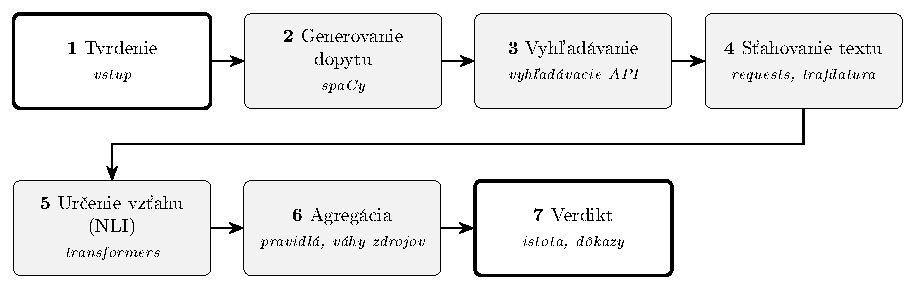
\includegraphics[width=\textwidth]{pipeline.pdf}
\caption{Schéma navrhovaného pipeline: z tvrdenia sa postupne získa
vyhľadávací dopyt, zdroje a ich plný text, vzťah textu k tvrdeniu
a nakoniec verdikt s mierou istoty a dôkazmi.}
\label{fig:pipeline}
\end{figure}

\subsection{Moduly 1--2: Vstup a generovanie vyhľadávacieho dopytu}

Vstupom je jedno tvrdenie v angličtine. Tvrdenie obsahuje slová
(predložky, spojky, pomocné slovesá), ktoré pri vyhľadávaní prekážajú.
Základný systém AVeriTeC preto vyhľadáva podľa skrátenej verzie
tvrdenia, ktorá ponecháva len slovesá, podstatné mená a prídavné mená
\cite{schlichtkrull2023averitec}. Rovnaký princíp použijeme aj my:
knižnica spaCy určí slovné druhy a pomenované entity a do dopytu sa
zaradia podstatné mená, vlastné mená, čísla, slovesá a prídavné mená.
Kvalita dopytu je pre vyhľadávanie podstatná: autori AVeriTeC uvádzajú, že
vyhľadávanie podľa tvrdenia a vygenerovaných otázok našlo užitočné
dôkazy v 9 z 20 preskúmaných prípadov, kým s referenčnými otázkami
v 16 z 20 \cite{schlichtkrull2023averitec}. Ako základná línia na
porovnanie slúži odstránenie stop-slov, voliteľne sa zváži aj
KeyBERT, ktorý vyberá frázy podľa významu celej vety.

\subsection{Moduly 3--4: Vyhľadávanie a sťahovanie textu}

Dopyt sa odošle do vyhľadávacieho API komerčného poskytovateľa (vyberie
sa podľa dostupnosti bezplatného prístupu), ktoré vráti zoznam adries URL
a krátkych úryvkov. Pre každú adresu sa stiahne HTML, pomocou knižnice
\texttt{trafilatura} sa z neho extrahuje hlavný text bez navigácie
a reklám a nedostupné stránky sa preskočia. Odpovede vyhľadávania
a stiahnuté texty sa ukladajú do vyrovnávacej pamäte, aby sa pri
opakovaných experimentoch nevyčerpával limit API a aby všetky porovnávané
varianty systému pracovali s tými istými stránkami.

\subsection{Modul 5: Určenie vzťahu medzi tvrdením a textom}

Stiahnutý text sa rozdelí na vety. Pre každú dvojicu (tvrdenie, veta)
model NLI určí jednu z troch tried: potvrdzuje, vyvracia, nesúvisí,
spolu s pravdepodobnosťou každej z nich. Použije sa anglický predtrénovaný
model založený na architektúre DeBERTa-v3 \cite{he2023debertav3}
dotrénovaný na korpuse MultiNLI \cite{williams2018mnli} cez knižnicu
\texttt{transformers}, takže netreba trénovať vlastný model. Do ďalšieho
spracovania idú len vety s pravdepodobnosťou nad prahom, ktorý sa nastaví
na časti trénovacej množiny datasetu AVeriTeC. Obmedzuje sa tým chybné označenie viet, ktoré len
dopĺňajú kontext, ako vyvracajúcich; tento problém sa objavil pri
základnom systéme AVeriTeC \cite{schlichtkrull2023averitec}.

\subsection{Moduly 6--7: Agregácia a výstup}

Základná agregácia vychádza z pravidla použitého v základnom systéme
AVeriTeC \cite{schlichtkrull2023averitec}: ak sú medzi dôkazmi aj
potvrdzujúce, aj vyvracajúce, verdikt je protichodné dôkazy; ak len
potvrdzujúce, potvrdené; ak len vyvracajúce, vyvrátené; inak nedostatok
informácií. Rozšírená verzia váži každý dôkaz mierou istoty modelu
a dôveryhodnosťou zdroja, ktorá sa odhadne podľa kategórie domény (napr.
vládne a akademické domény, spravodajské weby, sociálne siete a blogy),
aby niekoľko slabých zdrojov neprevážilo kvalitné. Výstupom je verdikt,
celková miera istoty a zoznam dôkazov s adresami zdrojov. Zoznam dôkazov
je len základnou formou zdôvodnenia, ktorá neodhaľuje celé uvažovanie
systému \cite{guo2022survey}. Prvá verzia používa konzolové rozhranie,
jednoduché webové rozhranie je voliteľné.

% ------------------------------------------------------------------
\section{Experimentálne vyhodnotenie}

\subsection{Dáta}

Na vyhodnotenie sa použije dataset AVeriTeC
\cite{schlichtkrull2023averitec}, ktorý obsahuje reálne tvrdenia
s dôkazmi z webu a pri ktorého tvorbe sa autori snažili obmedziť dôkazy
na dokumenty zverejnené pred vznikom tvrdenia. Verdikty datasetu
(potvrdené, vyvrátené, nedostatok informácií, protichodné dôkazy)
zodpovedajú výstupom systému. Dataset je nevyvážený: vyvrátené tvrdenia
tvoria približne 61 až 62~\% validačnej a testovacej množiny
\cite{schlichtkrull2023averitec}. Parametre systému (napr. prah v module~5) sa nastavia na časti trénovacej
množiny a vyhodnotenie prebehne na validačnej množine datasetu. Vyhodnocuje sa na náhodnej podmnožine
tvrdení s pevným semienkom generátora náhodných čísel, ktorej veľkosť
závisí od limitov vyhľadávacieho API.

Tvrdenia v datasete pochádzajú z fact-checkov z rokov 2020 až 2021, preto
by vyhľadávanie mohlo nájsť samotný fact-check s hotovým verdiktom. Aby sa
tomu zabránilo, zo zdrojov sa vylučujú weby fact-checkingových organizácií
\cite{schlichtkrull2023averitec}. Úplne vylúčiť únik verdiktu sa však nedá,
pretože ho môžu prebrať aj iné články.

\subsection{Metriky}

Kvalita verdiktov sa meria presnosťou (\textit{accuracy}), makro
F1-skóre a maticou zámen, aby bolo vidno chovanie pre každú triedu. Pre
nevyváženosť datasetu je hlavnou metrikou makro F1-skóre.

\subsection{Porovnávané systémy}

\begin{enumerate}
  \item \textbf{Základný pipeline}: navrhnutý systém s pravidlovou
        agregáciou.
  \item \textbf{Rozšírený pipeline}: agregácia vážená dôveryhodnosťou
        zdrojov.
  \item \textbf{Prístup založený na LLM} : reimplementácia
        agenta podľa \cite{nath-agent} v jazyku Python, ktorý určuje
        verdikt nad úryvkami z výsledkov vyhľadávania.
\end{enumerate}

Všetky porovnávané systémy dostanú rovnaké tvrdenia a rovnaké uložené
výsledky vyhľadávania; líšia sa tým, ako s nimi naložia.

\subsection{Ablačné experimenty}

Prínos jednotlivých častí sa overí ich vypnutím: porovnanie plného textu
stránok s úryvkami (cieľ~2) a porovnanie pravidlovej agregácie s váženou
(cieľ~3). Súčasťou vyhodnotenia je aj kvalitatívna analýza chýb na
vybraných príkladoch.

\subsection{Obmedzenia}

Dôveryhodnosť zdrojov sa odhaduje len podľa kategórie domény, čo je hrubé
priblíženie. Dataset obsahuje len anglické tvrdenia. Pri voliteľnom
porovnaní s LLM treba počítať s tým, že model mohol počas trénovania vidieť
aj tvrdenia z datasetu, čo môže skresliť výsledok.

% ------------------------------------------------------------------
\section{Použité technológie}

Systém sa implementuje v jazyku Python. Použité nástroje:
\begin{itemize}
  \item \texttt{spaCy} -- určovanie slovných druhov a rozpoznávanie
        pomenovaných entít pri generovaní vyhľadávacieho dopytu,
  \item API komerčného poskytovateľa vyhľadávania na webe,
  \item \texttt{requests} a \texttt{trafilatura} -- sťahovanie stránok
        a extrakcia hlavného textu,
  \item \texttt{transformers} a \texttt{PyTorch} -- modely NLI,
  \item \texttt{scikit-learn} -- výpočet metrík,
  \item voliteľne API veľkého jazykového modelu -- len pre porovnávaný
        prístup podľa \cite{nath-agent},
  \item Git a LaTeX -- správa kódu a dokumentácie.
\end{itemize}

% ------------------------------------------------------------------

\bibliographystyle{plain}
\bibliography{references}

\end{document}